\section{Hiện thực hệ thống} \label{sec:hienthuchethong}
Trong phần này, chúng tôi xin trình bày chi tiết về kỹ thuật cách rút trích các đặc trưng, hiện thực bộ phân loại cũng như tích hợp các yếu tố đó vào hệ thống. 
Chúng tôi hiện thực hệ thống bằng ngôn ngữ lập trình Python, phiên bản 2.7

\subsection{Thư viện và công cụ sử dụng}
Chúng tôi sử dụng các thư viện: UMLS, NLTK và Scikit-learn, cùng một số thư viện khác. Tất cả các thư viện đều là mã nguồn mở và miễn phí.
\subsubsection*{MetaMap}
MetaMap cung cấp 3 phương pháp cơ bản để sử dụng công cụ:
\begin{itemize}
\item Tương tác trực tiếp thông qua giao diện web\footnote{https://ii.nlm.nih.gov/Interactive/UTS\_Required/metamap.shtml} (\term{Use MetaMap Interactively}): MetaMap cung cấp giao diện web (hình~\ref{fig:mmweb}) giúp người dùng, đặc biệt là người mới sử dụng, có cái nhìn trực quan nhất về cách MetaMap hoạt động bao gồm cấu trúc dữ liệu đầu vào và đầu ra, những tùy chọn và cách các tùy chọn này ảnh hưởng đến kết quả phân tích. Tuy nhiên, mỗi lần gửi dữ liệu lên máy chủ MetaMap thông qua giao diện web này, MetaMap giới hạn dữ liệu đầu vào chỉ có một tập tin dữ liệu dạng text chứa không quá 10000 ký tự vì thế không thể sử dụng cách này cho những mẩu dữ liệu quá dài. Hơn nữa việc gửi và nhận kết quả trực tuyến thông qua mạng nên không đảm bảo tốc độ xử lý và bảo mật dữ liệu. Với những hạn chế vừa nêu, sau khi đã làm quen với cách hoạt động của MetaMap, người dùng có thể chọn 2 cách sau để tương tác với MetaMap.
\item Gửi dữ liệu lên máy chủ MetaMap\footnote{https://ii.nlm.nih.gov/Batch/UTS\_Required/metamap.shtml} (\term{Use Batch MetaMap}): người dùng có thể gửi bộ dữ liệu lên máy chủ của MetaMap (hình~\ref{fig:batchmm}), sau quá trình xử lý MetaMap sẽ trả kết quả về địa chỉ email người dùng cung cấp. Ưu điểm của phương pháp này là tốc độ xử lý nhanh do không có tương tác trong quá trình phân tích dữ liệu. Tuy nhiên khi xảy ra lỗi trong quá trình chạy thì khó phán đoán được lỗi xảy ra ở mẩu dữ liệu nào. 
\item Sử dụng MetaMap cục bộ (\term{Use MetaMap Locally}): Nếu người dùng muốn hoàn toàn kiểm soát dữ liệu của mình thì việc cài đặt MetaMap ngay trên máy tính cá nhân là lựa chọn tốt nhất. Ưu điểm của phương pháp này là tốc độ xử lý nhanh, không phụ thuộc vào hệ thống mạng do không cần gửi dữ liệu lên máy chủ MetaMap, đảm bảo quyền kiểm soát dữ liệu và khả năng điều chỉnh cấu trúc kết quả phù hợp với nhu cầu sử dụng. Tuy nhiên nhược điểm lớn của phương pháp này là tốn khá nhiều tài nguyên hệ thống và cần máy tính có cấu hình đủ mạnh để làm máy chủ cục bộ.
\end{itemize}

\begin{figure}[h]
\centering
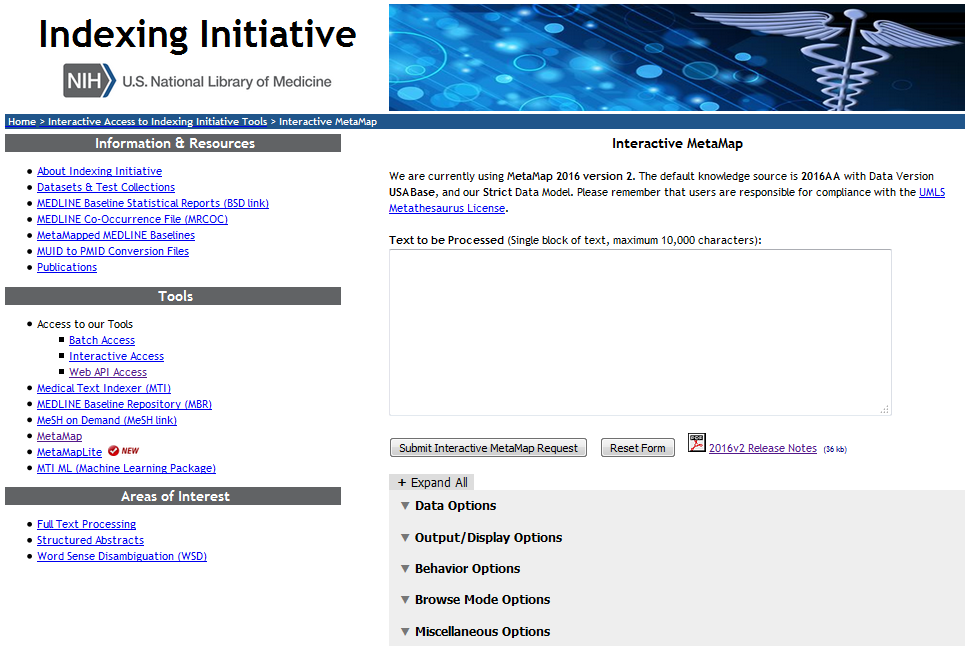
\includegraphics[scale=0.7]{../hinh/mmweb.png}
\caption{Giao diện web tương tác trực tiếp của MetaMap}
\label{fig:mmweb}
\end{figure}

Kết quả xử lý trả về như nhau khi dùng cả 3 phương pháp. Trong hệ thống phân loại chúng tôi đã dùng MetaMap cục bộ để tối đa khả năng điều chỉnh cấu trúc dữ liệu đầu ra. \\

\begin{figure}[h]
\centering
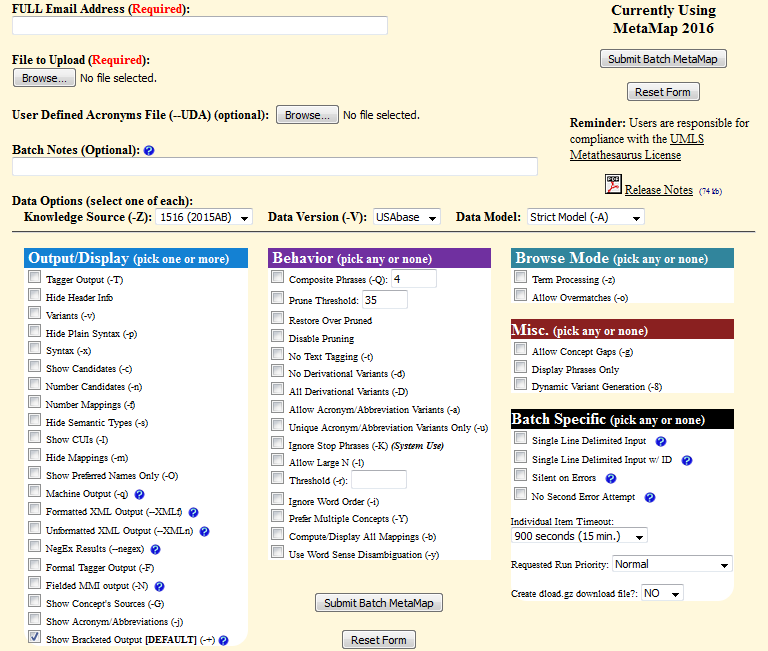
\includegraphics[scale=0.7]{../hinh/batchmm.png}
\caption{Batch MetaMap}
\label{fig:batchmm}
\end{figure}

Trong phạm vi luận văn, chúng tôi sử dụng công cụ MetaMap để xác định các nhãn y khoa tồn tại trong câu dữ liệu đầu vào. Chúng tôi đã tùy chọn bộ lọc nhãn từ vựng thuộc các nhóm ngữ nghĩa liên quan trực tiếp tới các triệu chứng, nguyên nhân, bệnh lý lâm sàng và cận lâm sàng như: \term{Pathologic Function}, \term{Disease or Syndrome}, \term{Mental or Behavioral Dysfunction}, \term{Cell or Molecular Dysfunction}, \term{Virus}, \term{Neoplastic Process}, \term{Anatomical Abnormality}, \term{Acquired Abnormality}, \term{Congenital Abnormality}, \term{Injury or Poisoning}.

Trong quá trình sử dụng MetaMap, chúng tôi chỉnh tùy chọn \textit{-negex} để lấy được kết quả đầu ra có phân tích phủ định. Đồng thời chúng tôi cũng xây dựng một chương trình con gọi là NegEx sử dụng giải thuật phân tích phủ định NegEx\footnote{https://code.google.com/p/negex/wiki/NegExAlgorithmDescription} để so sánh với kết quả từ MetaMap.

\subsubsection*{NLTK}
NLTK \cite{bird2009natural} là một \term{platform} xây dựng trên ngôn ngữ lập trình Python, cung cấp các công cụ để thao tác với văn bản. NLTK tích hợp hơn 50 \term{corpora} và các nguồn từ vựng (\term{lexicon}) như WordNet, SentiWordNet cùng các thư viện để xử lý ngôn ngữ tự nhiên, hỗ trợ: \term{tokenization}, \term{stemming}, \term{lemmination}, \term{parsing}. Ngoài ra NLTK đóng gói và cung cấp các giao diện lập trình (\term{API}) của các thư viện khác (thư viện Stanford NLP).\\

Trong nghiên cứu này, chúng tôi sử dụng NLTK như công cụ chính để thực hiện các bước tiền xử lý: tách câu, \term{tokenization}, \term{stemming}, \term{lemmination}
\subsubsection*{Scikit-learn}
Scikit-learn \cite{scikit-learn} là bộ thư viện về lĩnh vực Học máy trên nền tảng thư viện SciPy, sử dụng ngôn ngữ lập trình Python. Thư viện này cung cấp rất nhiều công cụ mà một bài toán Học máy cần dùng: Các giải thuật phân loại, hồi quy, phân cụm, \ldots; các công cụ tiền xử lý; các giải thuật thu giảm chiều; và các công cụ giúp lựa chọn, đánh giá mô hình.\\

Trong nghiên cứu này, chúng tôi sử dụng Scikit-learn là công cụ chính để hiện thực đặc trưng N-gram và giải thuật học máy SVM.

\subsubsection*{Các thư viện khác}
Ngoài 2 thư viện kể trên, chúng tôi sử dụng thêm:
\begin{itemize}
\item[•] NumPy giúp thao tác trên dữ liệu dạng vector.
\item[•] Pandas giúp đọc file, viết file và quản lý tập dữ liệu huấn luyện và dữ liệu để đánh giá.
\end{itemize}
\subsection{Hiện thực rút trích đặc trưng}
Trong phần này, chúng tôi sẽ trình bày cách thức hiện thực để từ một câu văn chuyển thành một vector, hoặc từ danh sách các câu chuyển thành một mảng 2 chiều. Từ đó làm input cho giải thuật học máy SVM
\subsubsection*{Đặc trưng N-gram}
Scikit-learn cung cấp các công cụ để làm việc với dữ liệu dạng text. Trong số này, chúng tôi sử dụng module sklearn.feature\_extraction.text.CountVectorizer để hiện thực đặc trưng N-gram. Như mô tả ở mục \ref{sec:ngram}, n-gram được trích xuất qua 2 bước:\\

Bước đầu tiên: Xây dựng tập từ vựng T. Scikit-learn cung cấp lớp CountVectorizer cho tác vụ này.
\begin{lstlisting}
vectorizer = CountVectorizer(input, min_df, binary, ngram_range)
\end{lstlisting}
Hàm khởi tạo CountVectorizer cung cấp 17 tham số, tuy nhiên, trong nghiên cứu này chúng tôi chỉ quan tâm đến 4 tham số, các tham số còn lại sử dụng giá trị mặc định:
\begin{description}
\item[input] Là các câu trong tập dữ liệu huấn luyện
\item[min\_df] Là số nguyên thể hiện số câu câu ít nhất chứa n-gram để n-gram đó được thêm vào tập từ vựng. Tham số này đã được giải thích chi tiết tại \ref{sec:ngram}
\item[binary] Là giá trị True hoặc False. Nếu $binary=True$, giải thuật sử dụng \term{vector nhị phân}\footnotemark, \footnotetext{2 khái niệm này được định nghĩa tại Mục \ref{sec:ngram}, phần Rút trích}
ngược lại sử dụng \term{vector số nguyên}\footnotemark
 \footnotetext{2 khái niệm này được định nghĩa tại Mục \ref{sec:ngram}, phần Rút trích}
 \item[ngram\_range] Là một \term{tuple}, có dạng $(a, b)$. Giải thuật sẽ sử dụng các loại n-gram từ a-gram đến b-gram. \\
 Ví dụ $ngram\_range = (1,3)$: Giải thuật sử dụng 3 loại n-gram: Uni-gram, bi-gram và tri-gram.
\end{description}

Bước thứ 2: xây dựng tập vector đại diện cho mỗi câu trong tập huấn luyện. Bước này được thực hiện bằng cách gọi hàm:
\begin{lstlisting}
vectors-ngram = vectorizer.transform(raw_documents).toarray()
\end{lstlisting}
trong đó $raw\_documents$ là tập hợp các câu. Hàm trên trả về một mảng 2 chiều $n*m$ với n là số lượng câu trong tập $raw\_documents$ và $m$ là kích thước của tập từ vựng
\subsubsection*{Đặc trưng Chang phrase}
Đặc trưng Change phrase ánh xạ một câu sang 1 vector 4 chiều. Trong phần hiện thực, chúng tôi định nghĩa hàm training\_change\_phrase:
\begin{lstlisting}
def training_change_phrase(raw_documents):
\end{lstlisting}
Hàm trả về mảng 2 chiều $n*4$ với $n$ là số lượng câu trong tập $raw\_documents$
\subsubsection*{Đặc trưng phủ định}
Chúng tôi sử dụng đồng thời 2 công cụ để trích xuất đặc trưng phủ định: MetaMap và NegEx. Việc này nhằm so sánh hiệu quả của 2 công cụ trên và chọn ra công cụ phù hợp hơn đối với nghiên cứu này.
\subsubsection*{SO-CAL}
Trong phần này, chúng tôi sử dụng phiên bản hiện thực của nghiên cứu \cite{taboada2011lexicon}. Nhóm tác giả của nghiên cứu \cite{taboada2011lexicon} đã hiện thực công cụ online để tính điểm số cho 1 đoạn văn, giao diện được mô tả như Hình \ref{fig:socal}.
\begin{figure}
\centering
\begin{subfigure}[b]{0.4\textwidth}
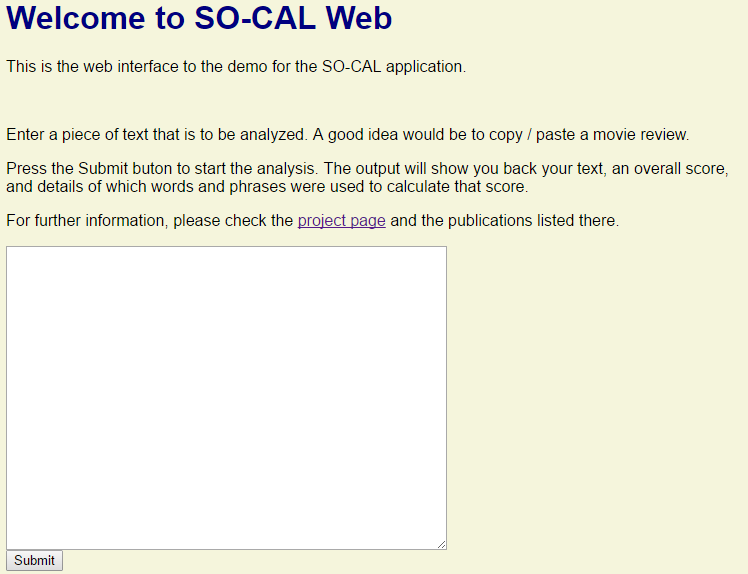
\includegraphics[scale=0.3]{../hinh/socal.png}
\caption{Nhập 1 đoạn text sau đó nhấp submit để chuyển đến trang kết quả}
\end{subfigure}
~
\begin{subfigure}[b]{0.4\textwidth}
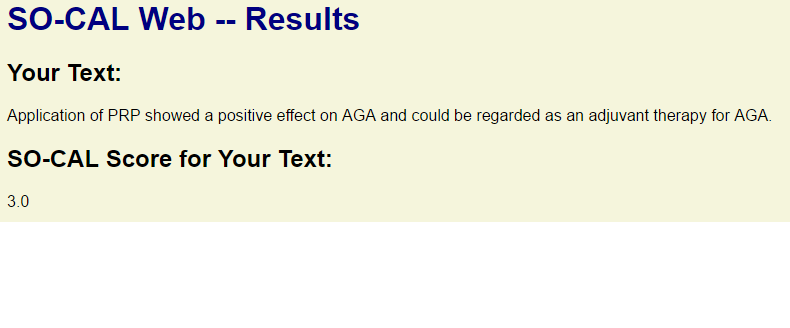
\includegraphics[scale=0.3]{../hinh/socal_result.png}
 \caption{Giao diện kết quả}
\end{subfigure}
\caption{Công cụ online để tính điểm SO-CAL} \label{fig:socal}
\end{figure}

Để tích hợp vào hệ thống, nhóm sử dụng package re trong Python, sử dụng phương thức HTTP POST để gửi yêu cầu lên trang web, sau đó parse phần kết quả trả về để lấy ra thông tin điểm số.
\subsection{Hiện thực bộ phân loại SVM}
\begin{figure}
\centering
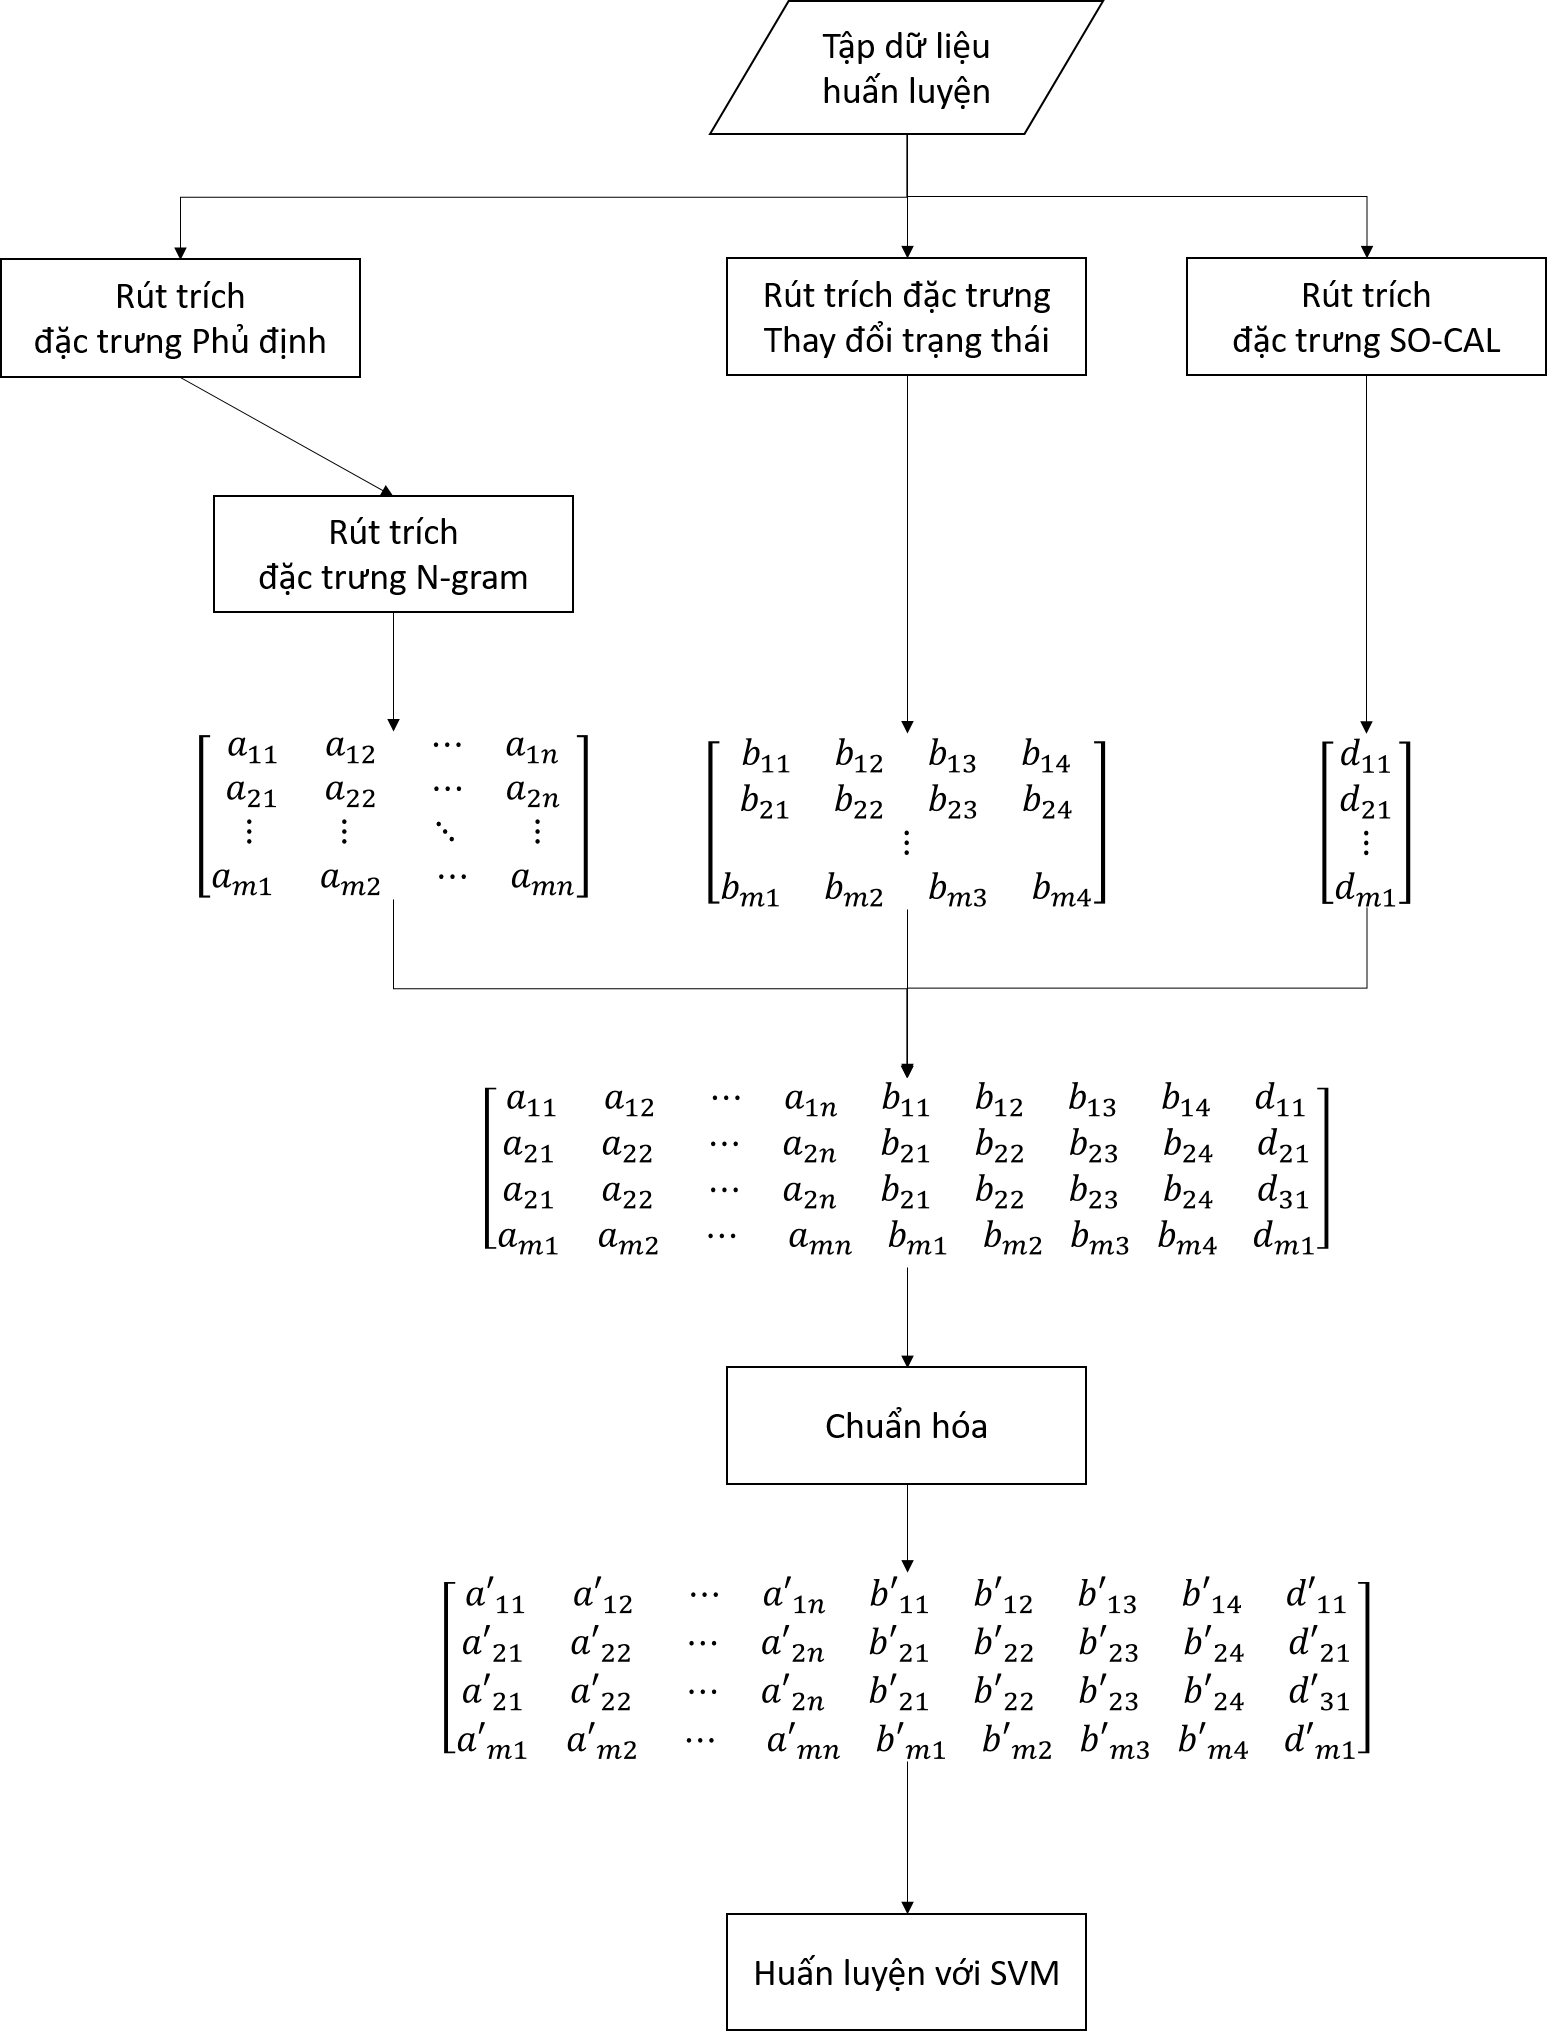
\includegraphics[scale=0.25]{../hinh/kethopdactrung.png}
\caption{Kết hợp các đặc trưng trước khi đưa vào SVM huấn luyện} \label{fig:ket-hop-dac-trung}
\end{figure}
Trước khi đưa vào giải thuật học máy SVM, các đặc trưng sau khi được rút trích như đã mô tả sẽ được kết hợp lại để với mỗi câu, chỉ có 1 vector đại diện. Mô hình kết hợp các đặc trưng được miêu tả như Hình \ref{fig:ket-hop-dac-trung}

